
%(BEGIN_QUESTION)
% Copyright 2012, Tony R. Kuphaldt, released under the Creative Commons Attribution License (v 1.0)
% This means you may do almost anything with this work of mine, so long as you give me proper credit

One of the pollutants generated by high-temperature combustion processes is {\it NO$_{x}$}: oxides of nitrogen.  NO$_{x}$ forms at high temperatures when nitrogen and oxygen gases in the combustion air combine to form nitrogen-oxygen molecules.  These molecules are considered a pollutant because they form nitric acid upon emission to the atmosphere, and they also contribute to the formation of smog.

A common method of mitigating NO$_{x}$ emissions is to recirculate exhaust gas into the intake of the combustion system.  Doing so reduces combustion temperature: a critical variable in the production of NO$_{x}$:

$$\includegraphics[width=15.5cm]{i01830x01.eps}$$

The reduction in combustion temperature approximately relates to exhaust gas recirculation by the following formula:

$$X = {{T_M - T} \over {T - T_W}}$$

\noindent
Where,

$X$ = Recirculation fraction (between 0 and 1, unitless)

$T_M$ = Maximum (theoretical) flame temperature

$T$ = Actual flame temperature

$T_W$ = Exhaust gas temperature

\vskip 10pt

Algebraically manipulate this equation to solve for $T$, then calculate the actual flame temperature  given a maximum theoretical temperature of 3100$^{o}$ F, an exhaust gas temperature of 480$^{o}$ F, and a recirculation factor of 22\%.

\vskip 10pt

Also, explain why we must have a recirculation {\it blower} installed at the location shown in the diagram, rather than a simple recirculation {\it valve}.

\vfil 

\underbar{file i01830}
\eject
%(END_QUESTION)





%(BEGIN_ANSWER)

This is a graded question -- no answers or hints given!

%(END_ANSWER)





%(BEGIN_NOTES)

We are asked to solve for $T$, and we see that $T$ appears twice in the equation, which means our task is to somehow collect all the $T$ terms on one side of the equation, consolidate them, and then solve for that one $T$.  

Perhaps the most challenging part of this manipulation is the step where we {\it factor} $T$ out of multiple terms containing $T$, as seen in the fifth step below, where $T + XT$ becomes $T(1 + X)$.  {\it Factoring} is the inverse operation to {\it distribution}: we can see this by distributing $T(1 + X)$ to get $T + TX$.

$$X = {{T_M - T} \over {T - T_W}}$$

$$X (T - T_W) = T_M - T$$

$$XT - XT_W = T_M - T$$

$$T + XT = T_M + XT_W$$

$$T (1 + X) = T_M + XT_W$$

$$T = {{T_M + XT_W} \over {1 + X}}$$

\vskip 10pt

$$T = {{3100 + (0.22)(480)} \over {1 + (0.22)}} = 2627.5 \hbox{ deg F}$$

\vskip 10pt

If a valve took the place of the recirculation blower shown, the flow would go the wrong direction: air to the exhaust, not exhaust back to the furnace inlet!

\vskip 30pt

Note: the formula shown in the question came from page 62 of Francis G. Shinskey's {\it Energy Conservation Through Control}, copyright 1978.

%INDEX% Control, strategies: NOx control by exhaust recirculation
%INDEX% Process: NOx control in furnace

%(END_NOTES)


